
\begin{frame}{Análise da Distribuição dos Pesos das Arestas}
    \begin{block}{Distribuição dos Pesos}
        \begin{itemize}
            \item \textbf{Distribuição dos Pesos das Arestas:} 
            \begin{itemize}
                \item Foco na análise de como os pesos das arestas (hierarquia das \textit{medalhas}) estão distribuídos na rede de atletas.
            \end{itemize}
            \item \textbf{Função de Distribuição Cumulativa (CDF):}
            \begin{itemize}
                \item Mostra a \textit{probabilidade acumulada} de um peso de aresta ser \textbf{menor ou igual} a um valor.
                \item Eixo X: Peso da Aresta; Eixo Y: Probabilidade Acumulada.
                \item Curva ascendente: indica a proporção de arestas com pesos menores que um dado valor.
            \end{itemize}
        \end{itemize}
    \end{block}
\end{frame}

\begin{frame}{Distribuição Cumulativa dos Pesos: Comparação Masculino vs Feminino}
    \framesubtitle{Análise Consolidada por Esporte e Gênero}
    \begin{center}
        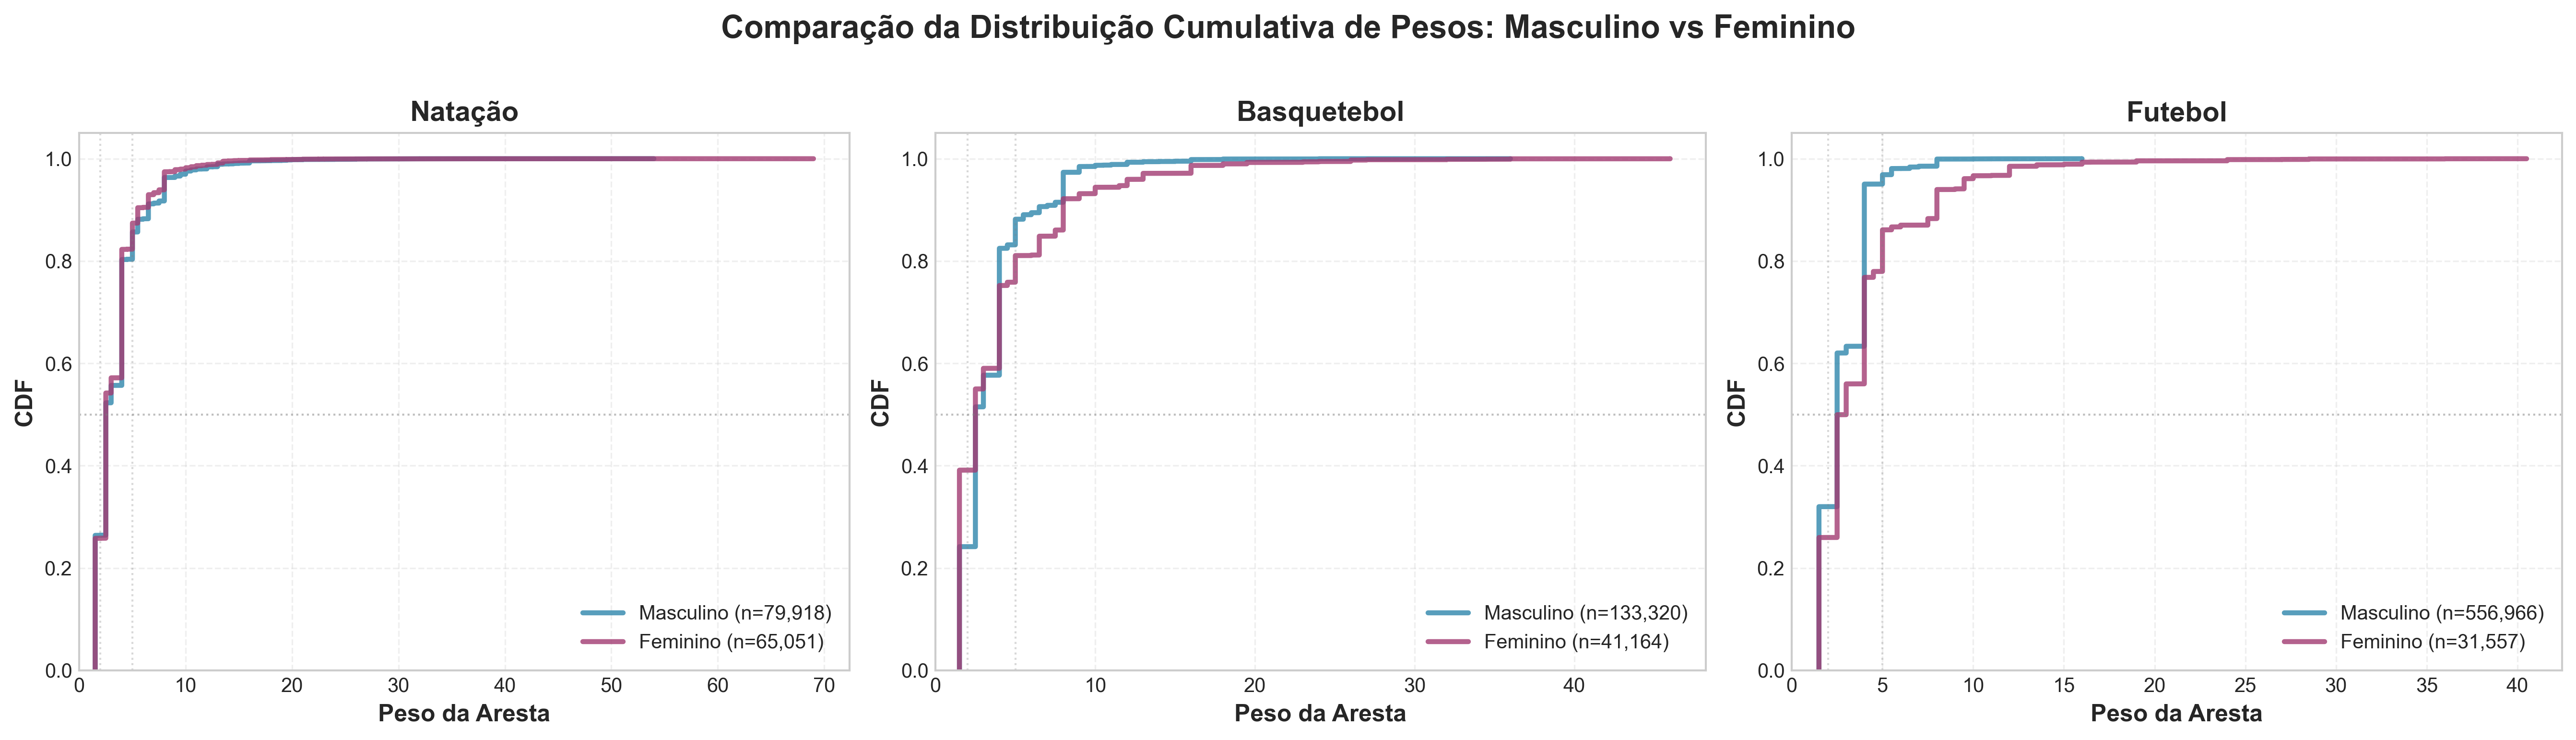
\includegraphics[width=0.95\textwidth]{figures/fig_edge_weight_cdf_comparison_mf.png}
    \end{center}

    \vspace{-0.3cm}
    \begin{block}{Observações Principais}
        \footnotesize
        \begin{itemize}
            \item \textbf{Distribuição similar} entre gêneros na maioria dos esportes
            \item \textbf{Maioria dos pesos $\leq$ 5}: concentração em diferenças pequenas de performance
            \item \textbf{Basketball F}: maior proporção de pesos baixos (39\% $\leq$ 2) vs M (24\%)
            \item Validação da modelagem: reflete proximidade competitiva esperada
        \end{itemize}
    \end{block}
\end{frame}

\begin{frame}{Resumo da Análise das CDFs e Validação da Modelagem}
    \begin{block}{Validação da Modelagem de Pódio Esportivo}
        \begin{itemize}
            \item As CDFs revelam que a maioria das arestas possui pesos baixos, refletindo pequenas diferenças de desempenho entre os atletas, o que é consistente com a proximidade competitiva esperada.
        \end{itemize}
    \end{block}
\end{frame}

\begin{frame}{Descoberta Estrutural: Fragmentação de Redes}
    \framesubtitle{Diferença Fundamental entre Tipos de Esportes}

    \begin{columns}[T]
        \begin{column}{0.48\textwidth}
            \begin{block}{Esportes Individuais}
                \footnotesize
                \textbf{Alta Fragmentação:}
                \begin{itemize}
                    \footnotesize
                    \item Athletics M: 269 componentes
                    \item Boxing M: 177 componentes
                    \item Swimming M: 66 componentes
                    \item Judo M: 45 componentes
                \end{itemize}

                \vspace{0.2cm}
                \textbf{Causa:}
                \begin{itemize}
                    \footnotesize
                    \item Especialização por modalidade
                    \item Categorias de peso isoladas
                    \item Velocistas $\neq$ Saltadores
                \end{itemize}
            \end{block}
        \end{column}

        \begin{column}{0.48\textwidth}
            \begin{block}{Esportes Coletivos}
                \footnotesize
                \textbf{Baixa Fragmentação:}
                \begin{itemize}
                    \footnotesize
                    \item Football F: 2 componentes
                    \item Basketball M: 3 componentes
                    \item Football M: 11 componentes
                \end{itemize}

                \vspace{0.2cm}
                \textbf{Causa:}
                \begin{itemize}
                    \footnotesize
                    \item Mesmos times ao longo do tempo
                    \item Rivalidades históricas
                    \item USA vs USSR, Brasil vs Argentina
                \end{itemize}
            \end{block}
        \end{column}
    \end{columns}

    \vspace{0.3cm}
    \begin{alertblock}{Contribuição Metodológica}
        \footnotesize
        \centering
        A estrutura da rede reflete a natureza da competição: individual = especialização, coletivo = continuidade
    \end{alertblock}
\end{frame}

